\chapter{WinRM: Windows Remote Management}

\url{https://www.hackingarticles.in/winrm-penetration-testing/}

\url{https://devops-collective-inc.gitbook.io/secrets-of-powershell-remoting/}
\section{Introduction}

Windows Remote Management (WinRM) is the Microsoft implementation of the
network protocol Web Services Management Protocol (WS-Management). It is a
network protocol based on XML web services using the Simple Object Access
Protocol (SOAP) used for remote management of Windows systems. It takes care of
the communication between Web-Based Enterprise Management (WBEM) and the
Windows Management Instrumentation (WMI), which can call the Distributed
Component Object Model (DCOM).

However, for security reasons, WinRM must be activated and configured manually
in Windows 10. Therefore, it depends heavily on the environment security in a
domain or local network where we want to use WinRM. In most cases, one uses
certificates or only specific authentication mechanisms to increase its
security. WinRM uses the {\bf TCP ports 5985 (HTTP) and 5986 (HTTPS)}.

Another component that fits WinRM for administration is {\bf Windows Remote Shell
(WinRS)}, which lets us execute arbitrary commands on the remote system. The
program is even included on Windows 7 by default. Thus, with WinRM, it is
possible to execute a remote command on another server.

Services like remote sessions using PowerShell and event log merging require
WinRM. It is enabled by default starting with the Windows Server 2012 version,
but it must first be configured for older server versions and clients, and the
necessary firewall exceptions created.

A handy tool that we can use for our password attacks is CrackMapExec, which
can also be used for other protocols such as SMB, LDAP, MSSQL, and others. We
recommend reading the official documentation for this tool to become familiar
with it.

\subsection{Archi}

\begin{figure}[!ht]
  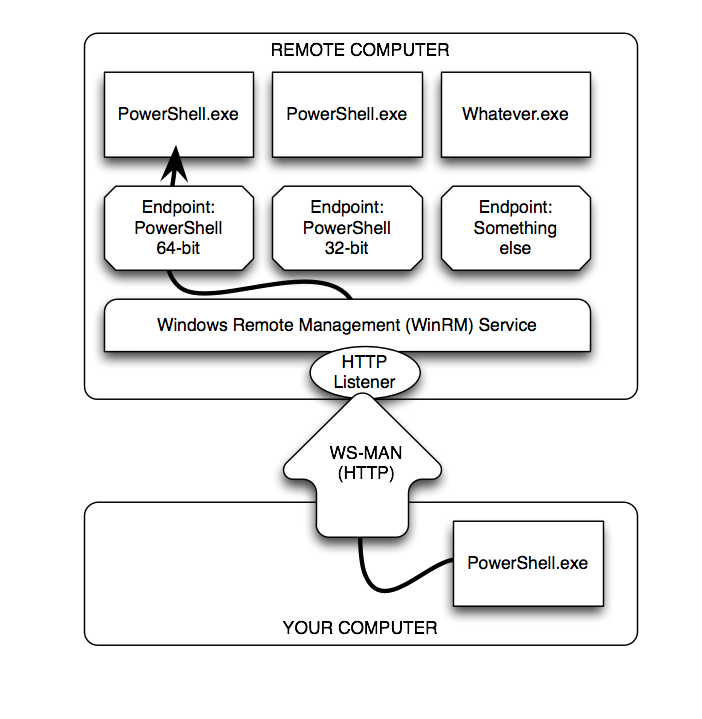
\includegraphics[width=\linewidth]{network/winrm/images/archi.png}
  \caption{winrm archi}
    \label{fig:winrm-archi}
\end{figure}
The computer will communicate via the WS-MAN, or Web Services for Management, protocol. This is an HTTP(S)-based protocol that can encapsulate a variety of different communications. We've illustrated this as using HTTP, which is Remoting's default configuration, but it could just as easily be HTTPS.

On the remote computer, the Windows Remote Management (WinRM) service runs. This service is configured to have one or more listeners. Each listener waits for incoming WS-MAN traffic on a specific port, each bound to a specific protocol (HTTP or HTTPS), and on specific IP addresses (or all local addresses).

When a listener receives traffic, the WinRM service looks to see which endpoint the traffic is meant for. For our purposes, an endpoint will usually be launching an instance of Windows PowerShell. In PowerShell terms, an endpoint is also called a session configuration. This is because, in addition to launching PowerShell, it can auto-load scripts and modules, place restrictions upon what can be done by the connecting user, and apply additional session specific settings not mentioned here.

\subsection{Listener}
\begin{verbatim}
Winrm create winrm/config/Listener?Address=*+Transport=HTTPS @{Hostname="xxx";CertificateThumbprint="yyy"}
\end{verbatim}

\subsubsection{Certificate Authentication}

\subsubsection{Modifying the TrustedHosts List}
The other option is to selectively disable the need for mutual authentication by providing your computer with a list of "trusted hosts."

\begin{verbatim}
Set-Item wsman:\localhost\client\trustedhosts *  
Set-Item wsman:\localhost\client\trustedhosts -value 'IP'  
\end{verbatim}

\subsubsection{Second Hop: CredSSP}
CredSSP must be enabled on your originating computer and the intermediate server you connect to. In PowerShell, on your originating computer, run:
\begin{verbatim}
Set-Item WSMAN:\localhost\client\auth\credssp -value $true
\end{verbatim}

On your intermediate server(s), you make a similar change to the above, but in a different section of the configuration:
\begin{verbatim}
Set-Item WSMAN:\localhost\service\auth\credssp -value $true
\end{verbatim}

Your domain policy must permit delegation of fresh credentials. In a Group Policy object (GPO), this is found in \verb+Computer Configuration > Policies > Administrative Templates > System > Credential Delegation > Allow Delegation of Fresh Credentials+. You must provide the names of the machines to which credentials may be delegated, or specify a wildcard like "*.ad2008r2.loc" to allow an entire domain. Be sure to allow time for the updated GPO to apply, or run Gpupdate on the originating computer (or reboot it).

When running a Remoting command, you must specify the \verb+-Authentication CredSSP+

Seem tedious and time-consuming to make all of those changes? There's a faster way. On the originating computer, run this:
\begin{verbatim}
Enable-WSManCredSSP -Role Client -Delegate <target_computer>
\end{verbatim}

on the intermediate computer:
\begin{verbatim}
Enable-WSManCredSSP -Role Server
\end{verbatim}

\subsubsection{Second Hop: Kerberos}
his allows ServerC to accept a delegated credential from ServerB
\begin{verbatim}
$ClientA = $env:COMPUTERNAME
$ServerB = Get-ADComputer -Identity ServerB
$ServerC = Get-ADComputer -Identity ServerC

Set-ADComputer -Identity $ServerC -PrincipalsAllowedToDelegateToAccount $ServerB
\end{verbatim}


\subsection{Endpoint}
There are two steps in setting up an endpoint:
\begin{enumerate}
    \item create a configuration file \verb+New-PSSessionConfigurationFile+
    \item registering that file \verb+Register-PSSessionConfiguration+
\end{enumerate}

An endpoint config can be:
\begin{itemize}
    \item 
        modified with \verb+Set-PSSessionConfiguration+
    \item displayed with \verb+Get-PSSessionConfiguration+
\end{itemize}

There are a number of reasons to create a custom endpoint (or configuration):
\begin{itemize}
    \item You can have scripts and modules auto-load whenever someone connects.
    \item You can specify a security descriptor (SDDL) that determines who is allowed to connect.
    \item You can specify an alternate account that will be used to run all commands within the endpoint - as opposed to using the credentials of the connected users.
    \item You can limit the commands that are available to connected users, thus restricting their capabilities.
\end{itemize}

\subsubsection{Security}

\begin{verbatim}
Set-PSSessionConfiguration -ShowSecurityDescriptorUI -Name Microsoft.PowerShell
get-PSSessionConfiguration
$PSSessionOption
\end{verbatim}
can restrict to Execute (Invoke)


\subsubsection{Accessing a specific endpoint}

\begin{verbatim}
Enter-PSSession -ComputerName <target_name> -Credential $creds -ConfigurationName <session_name>
\end{verbatim}

\subsection{WinRS}
Windows Remote Shell (WinRS) is a command line tool that is part of Windows 2008 and later. If WinRM is enabled this utility can be used to execute commands on a host remotely. The cmd argument will establish a new shell over command prompt.
\begin{verbatim}
winrs -r:http://WIN-2NE38K15TGH/wsman "cmd"
\end{verbatim}


\section{Footprint}

\subsection{nmap}
\begin{verbatim}
nmap -sV -sC  -p5985,5986 --disable-arp-ping -n

5985/tcp open  http    Microsoft HTTPAPI httpd 2.0 (SSDP/UPnP)
|_http-title: Not Found
|_http-server-header: Microsoft-HTTPAPI/2.0
Service Info: OS: Windows; CPE: cpe:/o:microsoft:windows

\end{verbatim}

\subsection{Enumeration}

The
\href{ https://docs.microsoft.com/en-us/windows/security/identity-protection/access-control/active-directory-security-groups#bkmk-remotemanagementusers}{Remote
Management Users} built-in security group.

tools to enumerate:
\begin{itemize}
    \item powerview~\ref{tool:powerview:Get-NetLocalGroupMember}
    \item bloodhound~\ref{tool:bloodhound:raw-query}
    \item {\bf LOL to write}
\end{itemize}


\section{Interaction}

\subsection{Evil-WinRM}
See~\ref{tool:evil-winrm}

\verb+evil-winrm -i <target-IP> -u <username> -p <password>+

\subsection{PowerShell}
See~\ref{tool:wlol:powershell:cmdlet:winrm-session}


\section{Brute Force}

\subsection{Metasploit}

Identify the WinRM Authentication Method: 

\begin{verbatim}
use auxiliary/scanner/winrm/winrm_auth_methods
\end{verbatim}

brute force : 

\begin{verbatim}
use auxiliary/scanner/winrm/winrm_login
set user_file /root/user.txt
set pass_file /root/pass.txt
set stop_on_success true
exploit
\end{verbatim}


\subsection{CrackMapExec}


\begin{verbatim}
crackmapexec <proto> <target-IP> -u <user or userlist> -p <password or passwordlist>
\end{verbatim}



\section{Links}
\begin{itemize}
    \item \url{https://docs.microsoft.com/en-us/windows/win32/winrm/portal}
    \item \url{https://docs.microsoft.com/en-us/windows/win32/winrm/ws-management-protocol}
    \item \url{https://en.wikipedia.org/wiki/Web-Based_Enterprise_Management}
    \item \url{https://docs.microsoft.com/en-us/windows/win32/wmisdk/wmi-start-page}
    \item \url{https://docs.microsoft.com/en-us/openspecs/windows_protocols/ms-dcom/4a893f3d-bd29-48cd-9f43-d9777a4415b0}
\end{itemize}

